\chapter{Monte Carlo Techniques and simulation strategy}
\label{c:MCtechniques}\index{Monte Carlo method}

This chapter explains the simulation strategy and the Monte Carlo
techniques used in \MCX. We first explain the concept of the x-ray
weight factor, and discuss the statistical errors in dealing with sums
of x-ray weights.  Secondly, we give an expression for how the weight
factor transforms under a Monte Carlo choice and specialize this
to the concept of direction focusing.  Finally, we present a way of
generating random numbers with arbitrary distributions.
More details are available in the Appendix concerning random numbers in the User manual.


\section{X-ray simulations}
%should talk about waveprop instead acceptance diagrams (although valid)
X-ray scattering beamlines are built as a series of optical elements.
Each of these elements modifies the beam characteristics (e.g. divergence,
wavelength spread, spatial and temporal distributions) in a way which, for simple
x-ray beam configurations, may be modelled with analytical methods. 

However, real x-ray beamlines consist of a large number of optical
elements, and this brings additional complexity by introducing strong
correlations between x-ray beam parameters like divergence and position - which
is the basis of the acceptance diagram method - but also wavelength and time.
The usual analytical methods, such as phase-space theory, then reach their
limit of validity in the description of the resulting effects.

%waveprop vs. 
In order to cope with this difficulty, Monte Carlo (MC) methods (for a general review, see Ref. \cite{James80}) may be
applied to the simulation of x-ray beamlines. The use of probability is commonplace in the description of microscopic
physical processes. Integrating these events (absorption, scattering, reflection, ...) over the x-ray trajectories
results in an estimation of measurable quantities characterizing the beamline. Moreover, using variance reduction
(importance sampling) where possible, reduces the computation time and gives better accuracy.

Implementations of the MC method for X-ray beamlines already exist, most
notable is probably \textit{SHADOW}\cite{welnak1994shadow}, originally developed by the late Franco
Cerrina and coworkers, now developed further by M. Sanchez Del Rio at the ESRF\cite{sanchez2011shadow3}\cite{shadow_website}.
Other implementations of the same concept are \textit{RAY}\cite{schaefers2008bessy} from BESSY and \textit{Xtrace}\cite{bauer2007simulation}.
hosted at ANKA

\subsection{Monte Carlo ray tracing simulations}
Mathematically, the Monte-Carlo method is an application of the law of large
numbers \cite{James80,Grimmett92}. Let $f(u)$ be a finite continuous integrable
function of parameter $u$ for which an integral estimate is desirable. The
discrete statistical mean value of $f$ (computed as a series) in the uniformly
sampled interval $a < u < b$ converges to the mathematical mean value of $f$
over the same interval.

\begin{equation}
\lim_{n \rightarrow \infty} \frac{1}{n} \sum_{i=1, a \leq u_i \leq b}^n f(u_i) = \frac{1}{b-a}\int_a^b f(u) du
\end{equation}

In the case were the $u_i$ values are regularly sampled, we come to the well
known midpoint integration rule. In the case were the $u_i$ values are randomly
(but uniformly) sampled, this is the Monte-Carlo integration technique. As
random generators are not perfect, we rather talk about
\emph{quasi}-Monte-Carlo technique. We encourage the reader to refer to James
\cite{James80} for a detailed review on the Monte-Carlo method.

\section{The x-ray weight}
\label{s:probweight}
A totally realistic semi-classical simulation will require that
each x-ray is at any time either present or lost.
On many beamlines the sheer abundance of x-ray photons makes it impractical to trace each
and every photon from the source. This is particularly the case at XFELs.
Additionally, only a very small fraction of the initial x-rays will ever be detected, and
simulations of this kind will therefore waste much time in dealing
with x-rays that never hit the detector.

A way of dealing with these issues and speed up calculations is to introduce
a x-ray "weight factor" for each simulated ray and to
adjust this weight according to the path of the ray.
If {\em e.g.}\ the reflectivity of a certain
optical component is 10\%, and only reflected x-rays ray are
considered later in the simulations, the x-ray
weight will be multiplied by 0.10 when passing this component,
but every x-ray is allowed to reflect in the component.
In contrast, the totally realistic simulation of the component
would require on average ten incoming x-rays for each reflected one.

Let the initial x-ray weight be $p_0$ and let us denote the weight
multiplication factor in the $j$'th component by $\pi_j$.  The resulting
weight factor for the x-ray ray after passage of the whole beamline
becomes the product of all contributions
\begin{equation}
\label{e:probprod}
p = p_n = p_0 \prod_{j=1}^n \pi_j .
\end{equation}
Each adjustement factor should be $0 < \pi_j < 1$, except in special
circumstances, so that total flux can only decrease through the simulation. For
convenience, the value of $p$ is updated (within each component)
during the simulation.

Simulation by weight adjustment is performed
whenever possible. This includes
\begin{itemize}
\item Transmission through filters and windows.
\item Reflection from monochromator (and analyser) crystals
 with finite reflectivity and mosaicity.
\item Reflections from mirrors.
\item Passage of a continuous beam through a chopper.
\item Scattering from all types of samples.
\end{itemize}

\subsection{Statistical errors of non-integer counts}
\label{s:staterror}
In a typical simulation, the result will consist of a
count of x-ray histories ("rays") with different weights. The
sum of these weights is an estimate of the mean number of x-rays
hitting the monitor (or detector) per second in a ``real'' experiment.
One may write the counting result as
\begin{equation}
\label{psum}
I = \sum_i p_i = N \overline{p} ,
\end{equation}
where $N$ is the number of rays hitting the detector and the horizontal bar
denotes averaging.
By performing the weight transformations, the (statistical)
mean value of $I$ is unchanged. However, $N$ will in general be enhanced,
and this will improve the accuracy of the simulation.

To give an estimate of the statistical error, we proceed as follows:
Let us first for simplicity assume that all the counted x-ray weights are
almost equal, $p_i \approx \overline{p}$,
and that we observe a large number of x-rays, $N \geq 10$.
Then $N$ almost follows a normal distribution
with the uncertainty $\sigma(N) = \sqrt{N}$
\footnote{This is not correct in a
situation where the detector counts a large fraction of the
x-rays in the simulation, but we will neglect that for now.}.
Hence, the statistical uncertainty of the observed intensity becomes
\begin{equation} \label{e:sigI1}
 \sigma(I) = \sqrt{N} \overline{p} = I / \sqrt{N} ,
\end{equation}
as is used in real x-ray experiments (where $\overline{p} \equiv 1$).
For a better approximation we return to Eq.~(\ref{psum}).
Allowing variations in both $N$ and $\overline{p}$,
we calculate the variance of the resulting intensity,
assuming that the two variables are independent:
\begin{equation}
\sigma^2(I) = \sigma^2(N) \overline{p}^2 + N^2 \sigma^2(\overline{p}) .
\end{equation}
Assuming as before that $N$ follows a normal distribution, we reach
$\sigma^2(N) \overline{p}^2 = N \overline{p}^2$.
Further, assuming that the individual weights, $p_i$,
follow a Gaussian distribution (which in some cases is far from the truth)
we have
$N^2 \sigma^2(\overline{p}) = \sigma^2(\sum_i p_i) = N \sigma^2(p_i)$
and reach
\begin{equation}
\sigma^2(I) = N \left( \overline{p}^2 + \sigma^2(p_i) \right).
\end{equation}
The statistical variance of the $p_i$'s is estimated by
$\sigma^2(p_i) \approx  (\sum_i p_i^2 - N \overline{p}^2) / (N-1)$.
The resulting variance then reads
\begin{equation}
\sigma^2(I) = \frac{N}{N-1} \left( \sum_i p_i^2 - \overline{p}^2  \right) .
\end{equation}
For almost any positive value of $N$, this is very well approximated
by the simple expression
\begin{equation}
\sigma^2(I) \approx \sum_i p_i^2 .
\end{equation}
As a consistency check, we note that for all $p_i$ equal, this reduces to
eq.~(\ref{e:sigI1})

In order to compute the intensities and uncertainties, the detector components
in \MCX\ will keep track of
$N=\sum_i p_i^0, I=\sum_i p_i^1$, and $M_2 = \sum_i p_i^2$.

\section{Weight factor transformations during a Monte Carlo
 choice}
When a Monte Carlo choice must be performed, {\em e.g.} when the
initial energy and direction of the x-ray ray is decided at the source,
it is important to adjust the x-ray weight so that the combined
effect of x-ray weight change and Monte Carlo probability
of making this particular choice
equals the actual physical properties we like to model.

Let us follow up on the simple example of transmission.
The probability of transmitting the real x-ray is $P$, but we make
the Monte Carlo choice of transmitting the x-ray every time:
$f_\mathrm{MC}=1$. This must be reflected on the choice of weight multiplier
$\pi_j$ given by the master equation
In the ``real'' semi-classical world, there is a distribution
(probability density) for the x-rays in the six dimensional
(energy, direction, position) space of
$\Pi(E,\Ombold,\mathbf{r}) = dP/(dE d\Ombold d^3\mathbf{r})$ depending upon
the source type and its parameters (such as gap, period, field strength etc. for an undulator).
In the Monte Carlo simulations, the six coordinates are for efficiency reasons
in general picked from another distribution:
$f_\mathrm{MC}(E,\Ombold,\mathbf{r}) \neq \Pi(E, \Ombold,\mathbf{r})$,
since one would {\em e.g.} often generate
only x-rays within a certain parameter interval.
However, we must then require that the weights are adjusted
by a factor $\pi_j$ (in this case: $j=1$) so that
\begin{equation} \label{probrule}
f_\mathrm{MC} \pi_j = P .
\end{equation}

This probability rule is general, and holds also if, e.g., it is decided to
transmit only half of the rays $(f_\mathrm{MC}=0.5)$.
An important different example
is elastic scattering from a powder sample,
where the Monte-Carlo choices are the particular powder line to scatter from,
the scattering position within the sample and the final x-ray direction
within the Debye-Scherrer cone.

\subsection{Direction focusing}
\index{Monte Carlo method!Direction focusing}
\label{s:focus}
An important application of weight transformation is direction focusing.
Assume that the sample scatters the x-rays in many directions.
In general, only x-rays in some of these directions will
stand any chance of being detected. These directions we call
the {\em interesting directions}.
The idea in focusing is to avoid wasting computation time on
x-rays scattered in the other directions.
This trick is an instance of what in Monte Carlo terminology
is known as {\em importance sampling}. % \cite{importance}.

If {\em e.g.} a sample scatters isotropically
over the whole $4\pi$ solid angle, and all interesting
directions are known to be contained within a certain
solid angle interval $\Delta \Ombold$, only these solid angles
are used for the Monte Carlo choice of scattering direction.
According to Eq.~(\ref{probrule}), the weight factor will then have
to be changed by the amount
$\pi_j = |\Delta \Ombold| / (4 \pi)$.
One thus ensures that the mean simulated intensity is unchanged
during a "correct" direction focusing, while a too narrow focusing will
result in a lower (\textit{i.e.} wrong) intensity, since
we cut x-rays rays that should have reached the final detector.

\begin{figure}[htb!]
\begin{center}
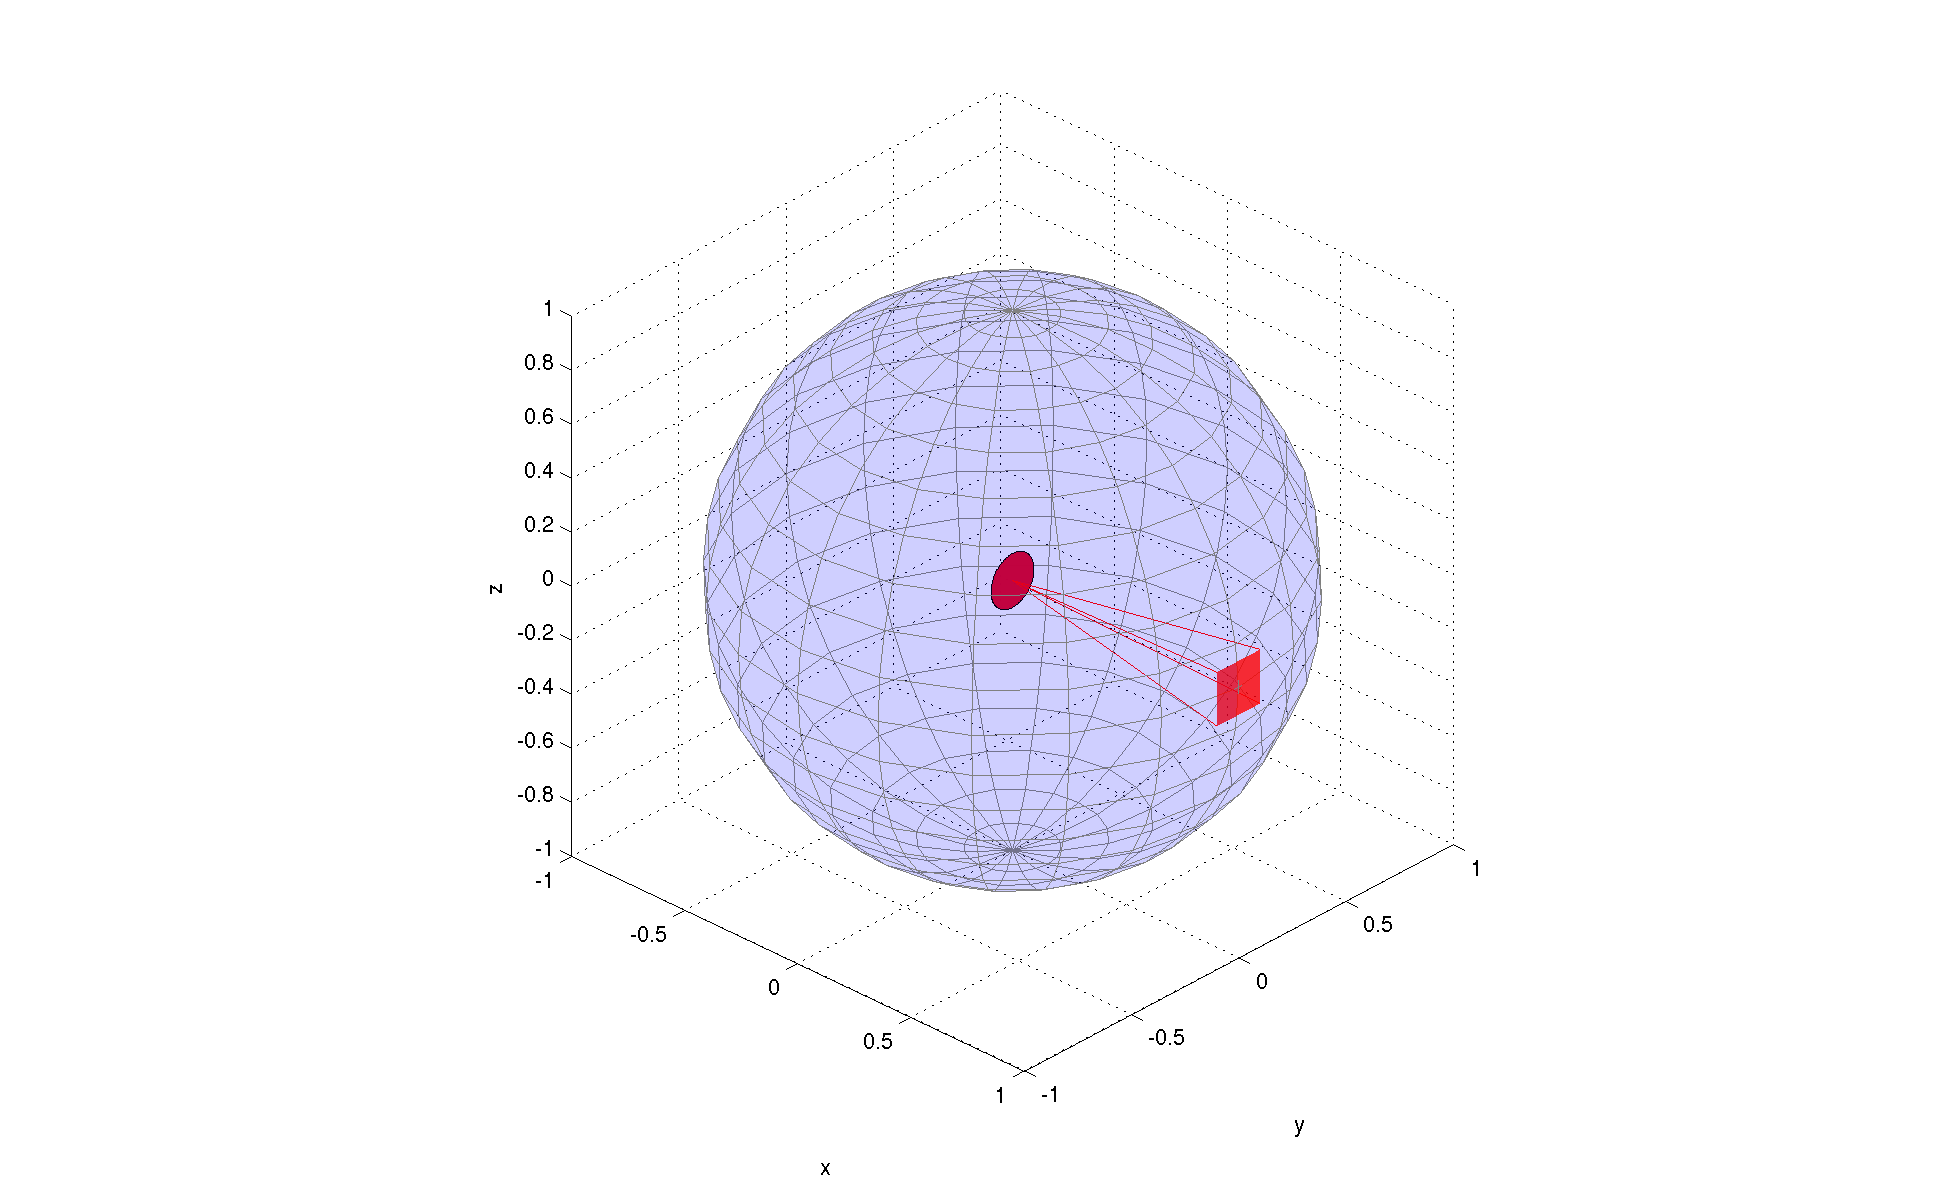
\includegraphics[width=.8\textwidth]{figures/focusing}
\end{center}
\caption{Illustration of the effect of direction focusing in \MCX. Weights of x-rays emitted into a certain solid angle are
  scaled down by the full unit sphere area.}
\label{fig:focusing}
\end{figure}

\section{Stratified sampling}
%\index{Monte Carlo method!Adaptive sampling}
\index{Monte Carlo method!Stratified sampling}
%Another strategy to improve sampling in simulations
%is \emph{adaptive importance sampling} (also called the variance reduction technique), % \cite{importance},
%where \MCX\ during the simulations will determine
%the most interesting directions and gradually change
%the focusing according to that.
%Implementation of this idea is
%found in the {\bfseries Source\_adapt} and {\bfseries Source\_Optimizer} components.
%, described in section~\ref{s:Source_adapt}.

One particular efficiency improvement technique is the so-called
\emph{stratified sampling}. It consists in partitioning the event distributions
in representative sub-spaces, which are then all sampled individualy. The
advantage is that we are then sure that each sub-space is well represented in
the final integrals. This means that instead of shooting $N$ events, we define
$D$ partitions and shoot $r=N/D$ events in each partition. We may define partitions so that they represent
'interesting' distributions, e.g. from events scattered on a monochromator or a
sample. The sum of partitions should equal the total space integrated by the
Monte Carlo method, and each partition must be sampled randomly.

In the case of \MCX, the stratified sampling is used when repeating events, i.e. when using the SPLIT
keyword in the TRACE section on beamline descriptions. We emphasize here that
the number of repetitions $r$ should not exceed the dimensionality of the Monte
Carlo integration space (which is $d=10$ for x-ray events) and the
dimensionality of the partition spaces, i.e. the number of random generators
following the stratified sampling location in the beamline.

\section{Accuracy of Monte Carlo simulations}
\index{Monte Carlo method!Accuracy}

When running a Monte Carlo, the meaningful quantities are obtained by
integrating random events into a single value (e.g. flux), or onto an histogram
grid. The theory \cite{James80} shows that the accuracy of these estimates is a
function of the space dimension $d$ and the number of events $N$. For large
numbers $N$, the central limit theorem provides an estimate of the relative
error as $1/\sqrt{N}$. However, the exact expression depends on the random
distributions.

\MCX\ uses a space with $d=12$ parameters to describe x-rays (position,
wavevector, weight, polarisation, phase, time). We show in Table \ref{t:mc_accuracy} a rough estimate of
the accuracy on integrals as a function of the number of records reaching the
integration point. This stands both for integrated flux, as well as for
histogram bins - for which the number of events per bin should be used for $N$.

\begin{table}
  \begin{center}
  {\let\my=\\
    \begin{tabular}{|c|c|}
    \hline
    Records       & Accurarcy \\
    \hline
    $10^3$ & 10 \% \\
    $10^4$ & 2.5 \% \\
    $10^5$ & 1 \% \\
    $10^6$ & 0.25 \% \\
    $10^7$ & 0.05 \% \\
    \hline
    \end{tabular}
    \caption{Accuracy estimate as a function of the number of statistical events used to estimate an integral with \MCX.}
    \label{t:mc_accuracy}
  }
  \end{center}
\end{table}

